\documentclass[titlepage]{article}

\title{NATuG User Manual}
\author{Wolf S. Mermelstein and William B. Sherman}

\usepackage{graphicx}
\usepackage{hyperref}
\usepackage{subcaption}
\usepackage{wrapfig}
\graphicspath{{resources/images}} % all graphics will come from the resources/images folder

\begin{document}
	\maketitle
	\tableofcontents 
	\newpage
	
	\section{Getting NATuG Running}
	
	The quick start guide is the fastest way to get NATuG running on any Mac, Windows, or Linux machine. These steps are by no means comprehensive, and are merely a guide to get the program running.
	
	\begin{figure}[h]
		\centering
		\label{fig:github-download-menu}
		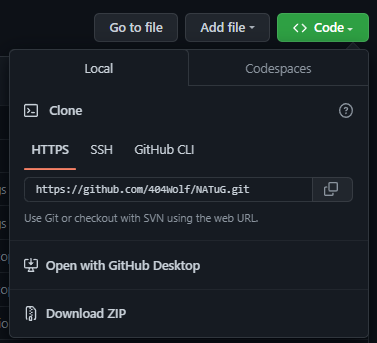
\includegraphics[width=2in]{github-download-menu.png}
		\caption{Github code download menu}
	\end{figure}
	
	\begin{enumerate}
		\item Visit \href{Python's download page}{www.python.org/downloads}, and then install the most recent version of Python for your operating system. NATuG has been confirmed to work on versions up to Python 3.11.1
		\item Go to the \href{NATuG’s Github page}{github.com/404Wolf/NATuG}, click the green "code" button, and then click "download ZIP." See Figure~\ref{fig:github-download-menu}.
		\item Open your computer’s terminal/console/command prompt. Enter the following commands, in the following order. 
		
		\begin{enumerate}
			\item “cd $<$filepath$>$” to enter the directory of the project. Generally this will be something along the lines of \mbox{cd C:/Users/Name/Downloads/NATuG-main,”} but it may vary based on operating system, where you download the folder, and the name of the folder. \label{enum:enter-directory}
			\item “python -m venv venv” to create a virtual environment for the needed libraries to go into.
			\item “venv\\Scripts\\activate” if you are on windows, or \nolinebreak{“source myenv/bin/activate”}	if you are on Mac/Linux, to enter into the virtual environment. You will know that you have successfully entered the virtual environment if the current line in terminal begins with “(venv).” \label{enum:activate-venv}
			\item “python -m pip install -r requirements.txt” to automatically install all the needed libraries. They may take a while to download. Once they have installed, when	loading NATuG in the future you can skip this step.
			\item “python -m launcher” to run the program. The first launch may take a bit while the code compiles. \label{enum:run-program}
		\end{enumerate}
	
		\item You should now be in NATuG! When running the program in the future, simply CD into the folder (step~\ref{enum:enter-directory}), enter the virtual environment (step~\ref{enum:activate-venv}), and run the program (step~\ref{enum:run-program}).
	\end{enumerate}

	\section{Overall Layout}
	
	NATuG’s interface consists of a main hub area, surrounded by two panels. There is a status bar at the bottom of NATuG, which provides helpful descriptions of what various buttons and input boxes do as you hover over them, and a file bar at the top of NATuG, which provides access to various cross-program functions.
	
	\begin{figure}[h]
		\centering
		\caption{The overall layout of NATuG}
		\label{program-layout}
		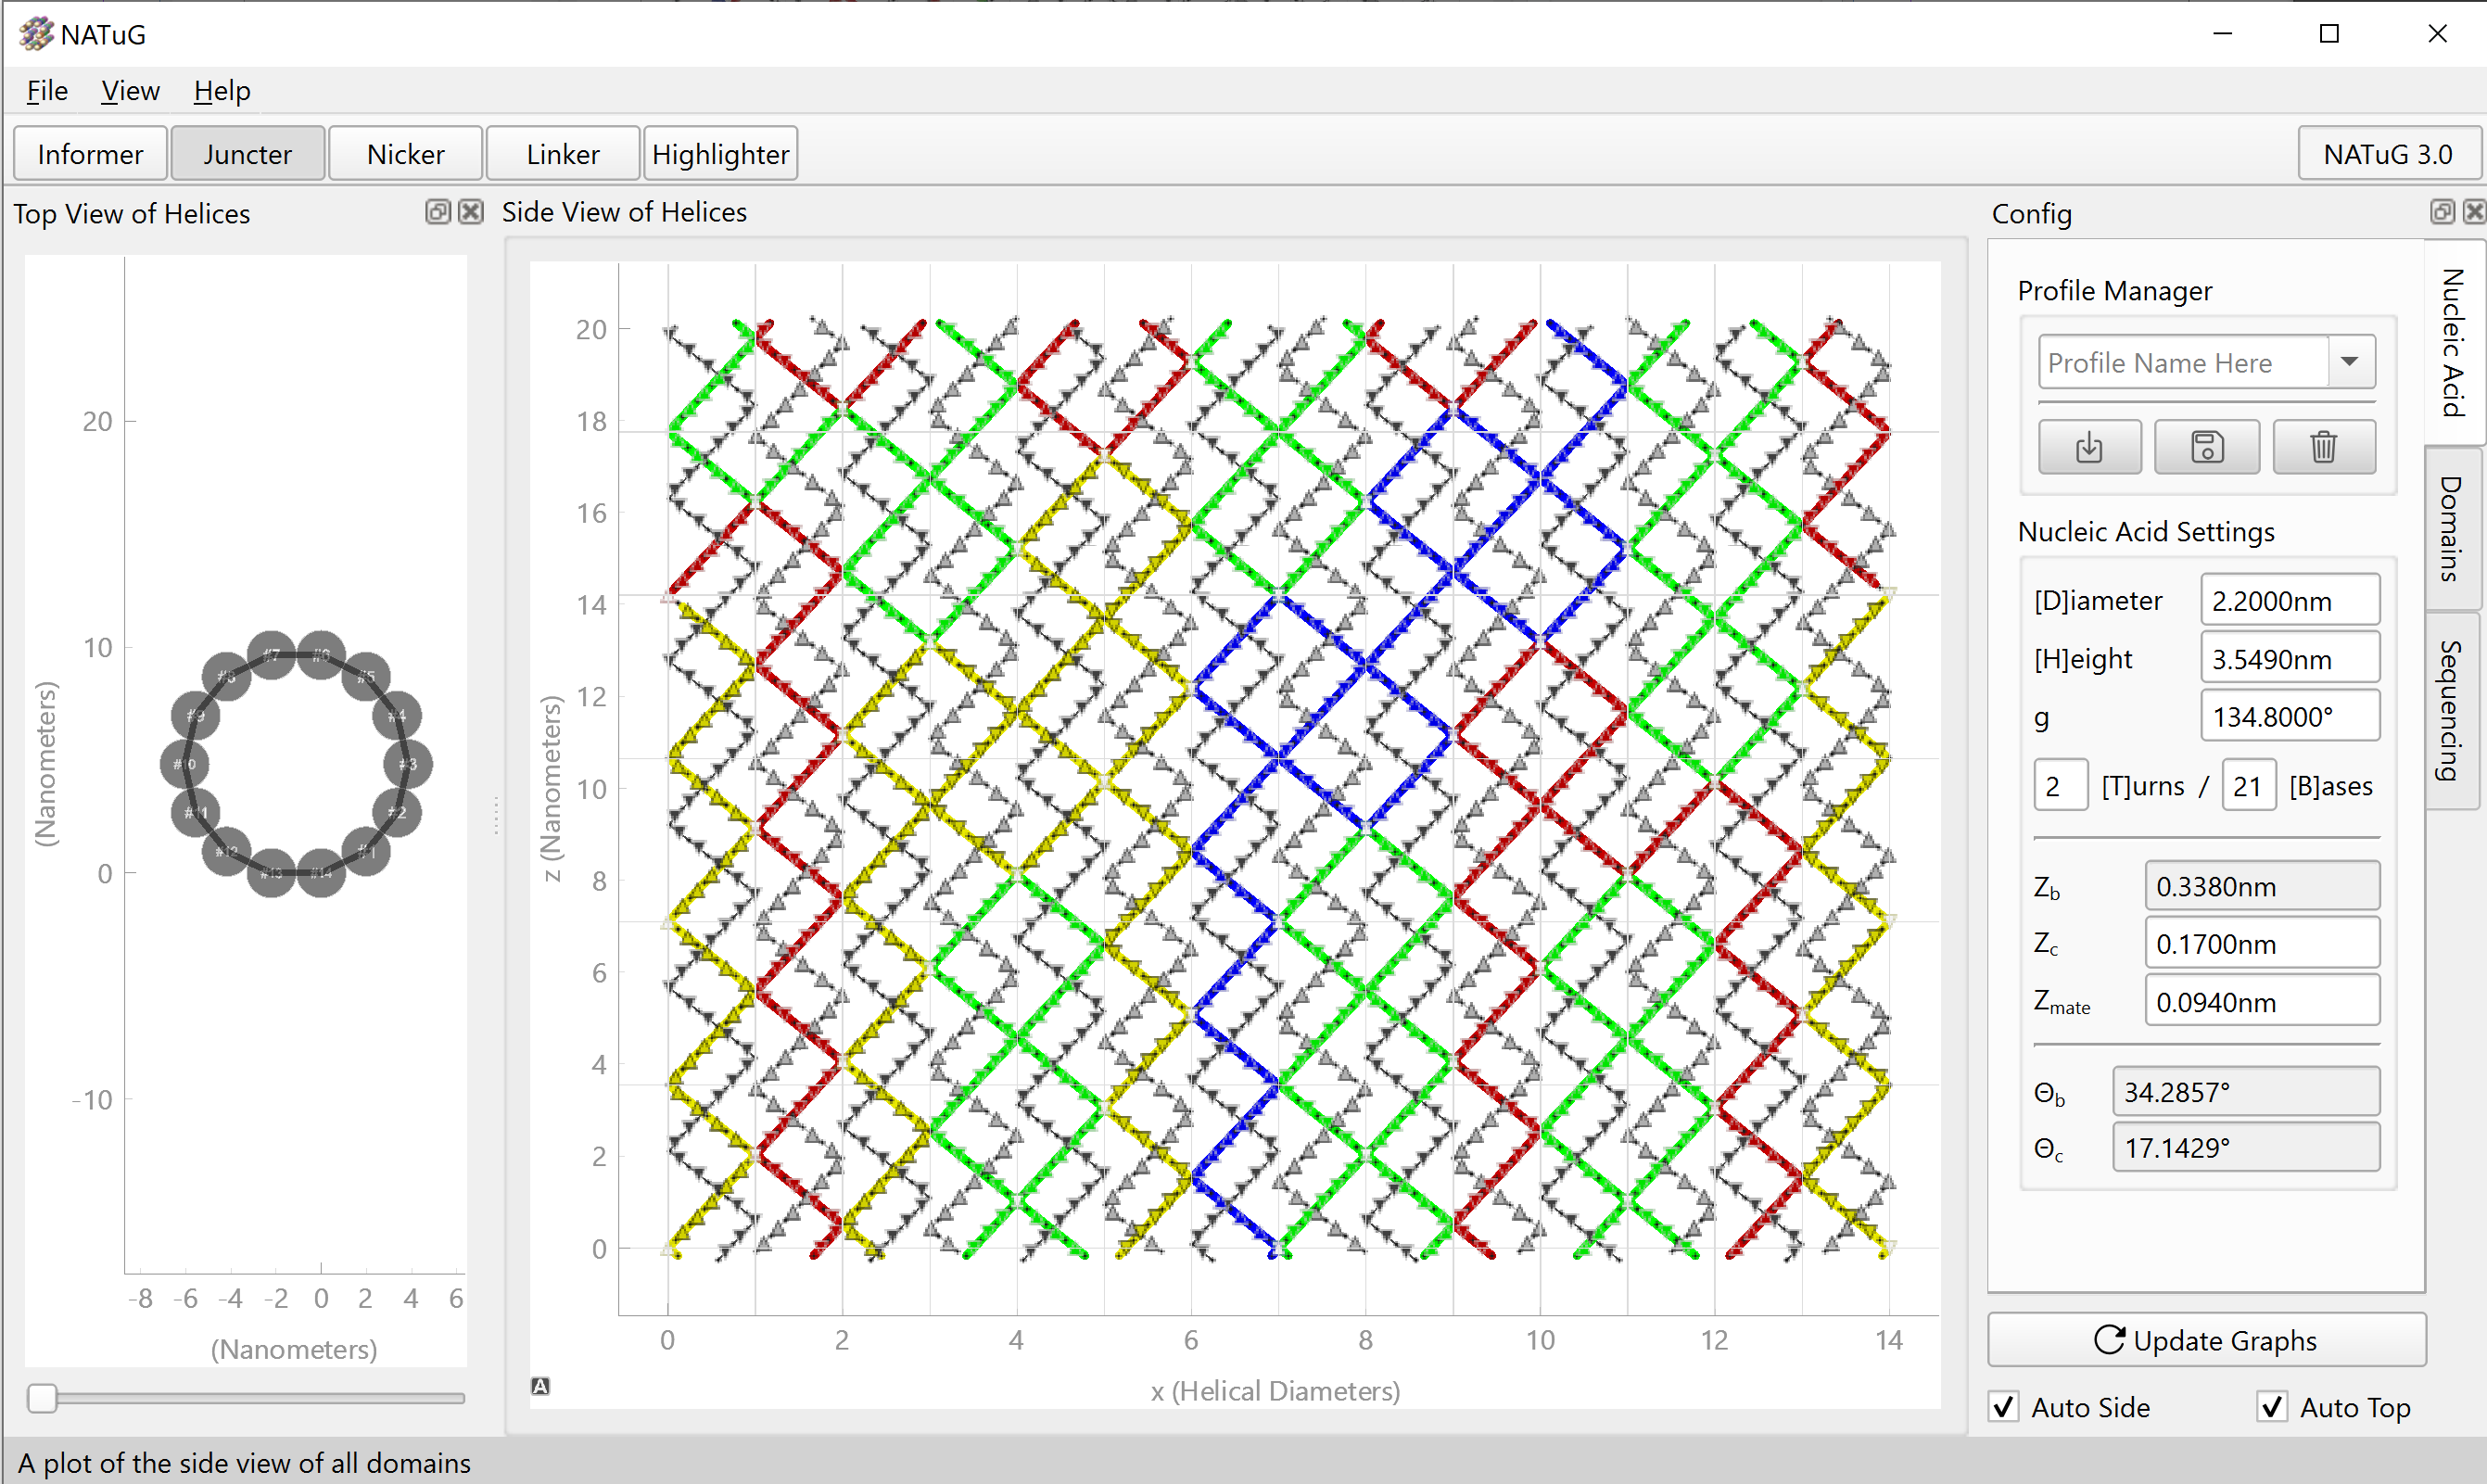
\includegraphics[width=5in]{program-layout.png}
	\end{figure}

	\subsection{Panels}
	NATuG has two panels: the Top View Panel and the Config Panel. Notes about panels:
	
	\begin{enumerate}
		\item Panels are all undockable. By clicking twice on the top area of a panel, or by dragging the panel away from the main window, or by clicking the  button, one can make a panel become its own window. To redock, click on the top of the panel twice, or drag the panel back into the main window. 
		\item Panels are hideable. By clicking the x button in the top corner of a panel, or by going to the file menu, “view,” and then the name of the panel you are trying to hide, you can hide the panel. To unhide a panel, go to the file menu, “view,” and then the name of the panel you are trying to unhide. 
	\end{enumerate}

	\subsection{Hub}
	NATuG’s main area, the “hub,” is another name for the area of the program where the Side View plot is located. Located directly above the Hub is the toolbar, where you can select the current mode of NATuG. Each mode changes what a left click does in the Side View plot.
	
	\section{Configuration Panel} \label{section:config-panel}
	The Config Panel contains most of the user input areas of NATuG. Within the panel are three primary modes: “Nucleic Acid,” “Domains,” and “Sequencing,” outlined in greater depth on the following pages. 
	
	To navigate between panels of the config panel, simply click on one of the tabs. Below are brief descriptions of the various tabs; however, each tab has a dedicated page as well.
	
	\textbf{Warning:} changing settings within the config panel will reset all current junctions, nicks, links, and highlights. Attempting to change settings when there exist any junctions, links, or highlights will result in a popup dialog that offers to save the current state of the Side View Plot, or cancel.
	
	\begin{figure}[h]
		\centering
		\includegraphics[width=3in]{"nucleic-acid-tab-activated.png"}
		\label{fig:nucleic-acid-tab-activated}
	\end{figure}

	The Nucleic Acid Tab is where one can customize the geometrical settings of the nucleic acid that they are creating a nanotube for. This defaults to B type DNA, and generally does not need to be changed. 

	\begin{figure}[h]
		\centering
		\includegraphics[width=3in]{"domains-tab-activated.png"}
		\label{fig:domains-tab-activated}
	\end{figure}

	The Domains Tab is where settings for the interior angles, strand switches, and the number of NEMids to generate are inputted. This section allows the user to actually define the shape of the nanotube.

	\begin{figure}[h]
		\centering
		\includegraphics[width=3in]{"sequencing-tab-activated.png"}
		\label{fig:sequencing-activated}
	\end{figure}

	The Sequencing Tab is where the user can apply bulk sequence actions to all the strands, and export sequences to a spreadsheet for synthesis. This is generally one of the later steps in the nanotube design process.
	
	\subsection{Graph Updating}
	
	By default, as changes are made within the various tabs of the Config Panel the Side View Plot and Top View Plot automatically update. To disable automatic updating for either plot, click either of the “Auto Side” or “Auto Top” buttons on the bottom of the Config panel. When automatic updating is disabled, the “Update Graphs” button must be clicked to refresh the plots. Manual updating can be useful for larger structures that take a long time to load.
	
	The current tab of the Config Panel determines what is currently plotted in the Side View Plot. When the current tab is either “Nucleic Acid” or “Domains” NEMids are plotted, and the mode of the Side View Plot is unrestricted. However, when “Sequencing” is active, nucleosides are plotted. When this is the case, only the “highlighter” and “informer” modes are enabled within the Side View Plot’s toolbar.
	
	\subsection{Nucleic Acid Tab}
	
	The Nucleic Acid Tab is the area in which all geometrical settings for the nucleic acid being used can be entered. All of NATuG’s computations utilize these constants, so only make changes if you know what you are doing.
	
	\subsubsection{Profile Manager}
	
	The profile manager lets you easily save and load various sets of nucleic acid settings. Using NATuG’s profile defaults will ensure that all the settings are correct, and you can also create your own profiles for future use.
	
	By default, NATuG includes common profiles, such as one for B type DNA. Profiles are saved internally, and can easily be loaded/retrieved, and .json files containing the profile data can be found within the saves/nucleic\_acid folder. These files are loaded when NATuG is booted, and can be modified directly. Additionally, when NATuG is closed, the last used settings are saved, and are automatically retrieved upon the next launch.
	
	To use the profile manager, enter the name of the profile you would like to save/load/delete into the “Profile Name Here” box, and click the respective button. For extended descriptions of what each button does, see below. When a profile manager box is disabled/gray consult the status bar for information as to why. For irreversible actions warnings will be shown.
	
	\begin{figure}[h]
		\caption{Various Profile Actions}
		
		\centering
		\begin{subfigure}{.3\textwidth}
			\centering
			\caption{The load profile button}
			
\includegraphics[width=1in]{load-profile-button.png}
			\label{fig:load-profile-button}
		\end{subfigure}%
		~
		\begin{subfigure}{.3\textwidth}
			\centering
			\caption{The save profile button}
			
\includegraphics[width=1in]{save-profile-button.png}
			\label{fig:save-profile-button}
		\end{subfigure}%
		~
		\begin{subfigure}{.3\textwidth}
			\centering
			\caption{The delete profile button}
			
\includegraphics[width=1in]{delete-profile-button.png}
			\label{fig:delete-profile-button}
		\end{subfigure}
	\end{figure}
	
	\paragraph{Load Profile}
	Load the profile with the currently chosen profile name. This requires a profile to already exist with the name chosen, and for the current settings to not be the same as the settings of that profile. (Icon~\ref{fig:load-profile-button})
	
	\paragraph{Save Profile}
	Save the profile with the currently chosen profile name, or, if there is already a profile with that name, overwrite the existing profile. The profile will be saved to a .json file within saves/nucleic\_acid after the program is closed. (Icon~\ref{fig:save-profile-button})
	
	\paragraph{Delete Profile}
	Delete the profile with the currently chosen profile name. This action is irreversible. Default profiles cannot be deleted. (Icon~\ref{fig:delete-profile-button})

	\subsubsection{Setting Descriptions}
	Below lies a list of all of the various Nucleic Acid settings that can be adjusted. Certain settings (the ones that are have an "(a)" in the table) are automatically determined based on other settings and cannot be user set.

	\begin{tabular}{|p{.5in}|p{1in}|p{.7in}|p{1.5in}|}
		\label{tab:setting-descriptions}
		\centering
		Input & Name & Data Type & Description \\
		\hline
		$D$ & Diameter & number & The diameter of a given domain in nanometers \\ \hline
		$H$ & Height & number & The height of one turn of the helical axes \\ \hline
		$g$ & Nucleoside-Mate Angle & number between 0 and 360 & The angle about the helical axis between a nucleoside and its Watson-Crick mate \\ \hline
		$T/B$ & Helical Turns per Bases & integers & There are T turns every B bases \\ \hline
		$Z_b$ (a) & Base Height & number & The height between two NEMids on a given helix \\ \hline
		$Z_c$ & Characteristic Angle & number & The height a helix climbs as it rotates through the characteristic angle \\ \hline
		$Z_{mate}$ & Nucleoside-Mate Height & number & Vertical distance between a NEMid and its mate on the other helix. \\ \hline
		$\theta_{c}$ (a) & Characteristic Angle & number between 0 and 360 & The smallest angle about the helical axis possible between two NEMids on the same helix. \\ \hline
		$\theta_{b}$ (a) & Interbase Angle & number between 0 and 360 & The angle that about the helical axis between two NEMids \\
	\end{tabular}
	
	\subsection{Domains}
	
	\begin{figure}[h]
		\centering
		\caption{Domains Config Table}
		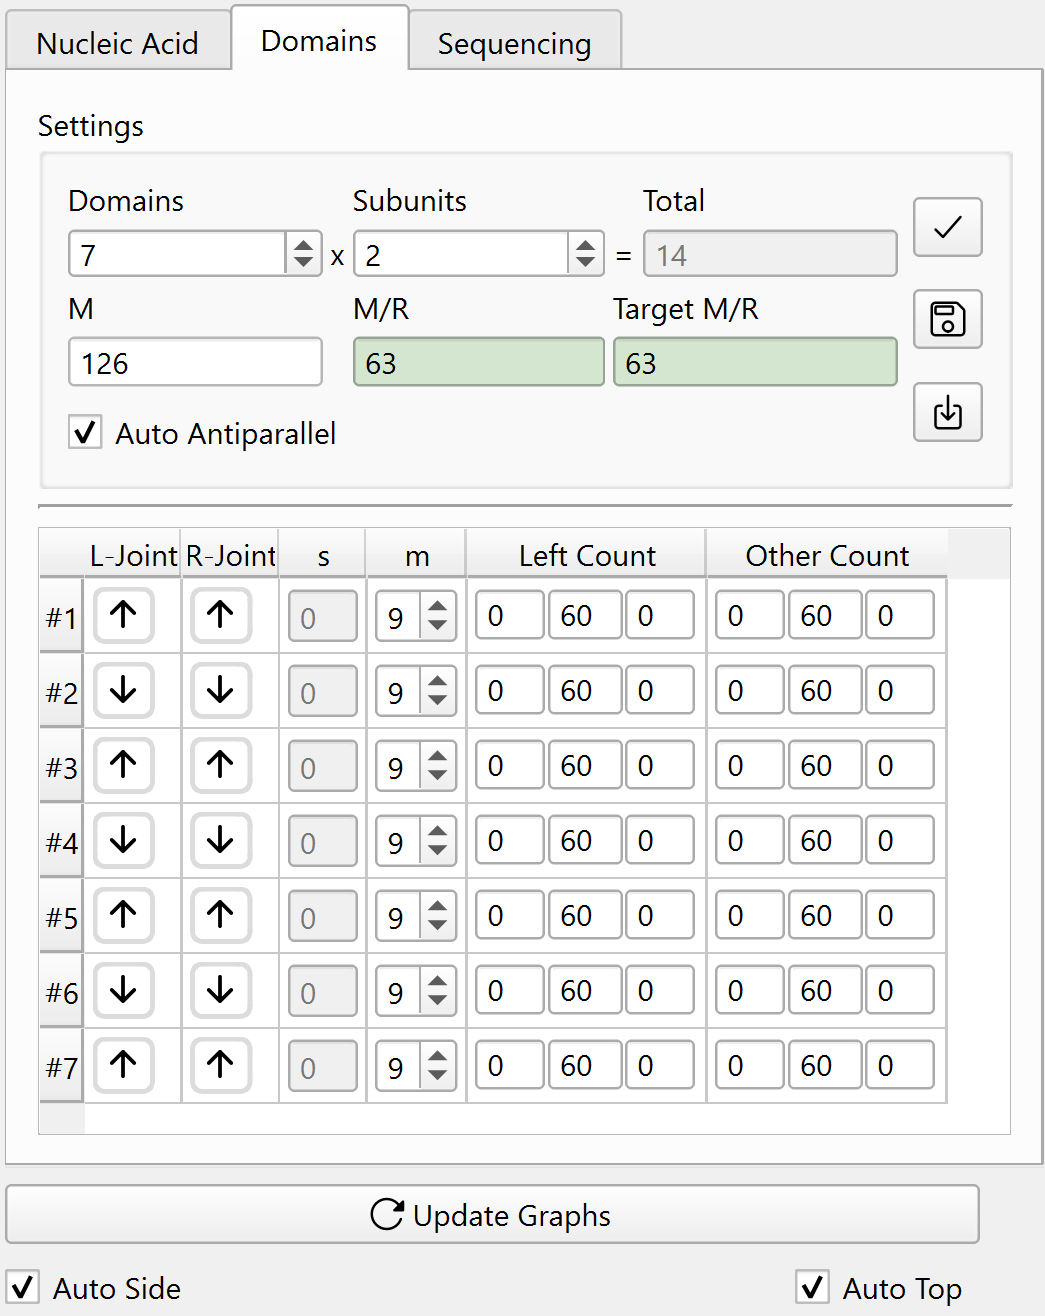
\includegraphics[height=2in]{domain-config-table.png}
		\label{fig:domain-config-table}
	\end{figure}

	The Domains Tab is the area in which all the settings for each helical domain can be set. The angles between each domain are what determine what the ultimate shape of the nanostructure will be. NATuG provides support for symmetrical designs, saving and loading designs, and provides tools for designing closed structures.
	
	\begin{itemize}
		\item "M" represents the sum of all of the little "m"s for each domain in the Table Area.
		\item "R" represents the number of subunits, and a green "M/R" box indicates that the tube is closed.
		\item To create sticky ends, adjust the left/rightmost boxes of the “Left/Other Count” columns. For more information, see "Settings Descriptions"
	\end{itemize}
	
	\subsection{Sequencing}
	
	\begin{figure}[h]
		\centering
		\caption{Sequencing Tab}
		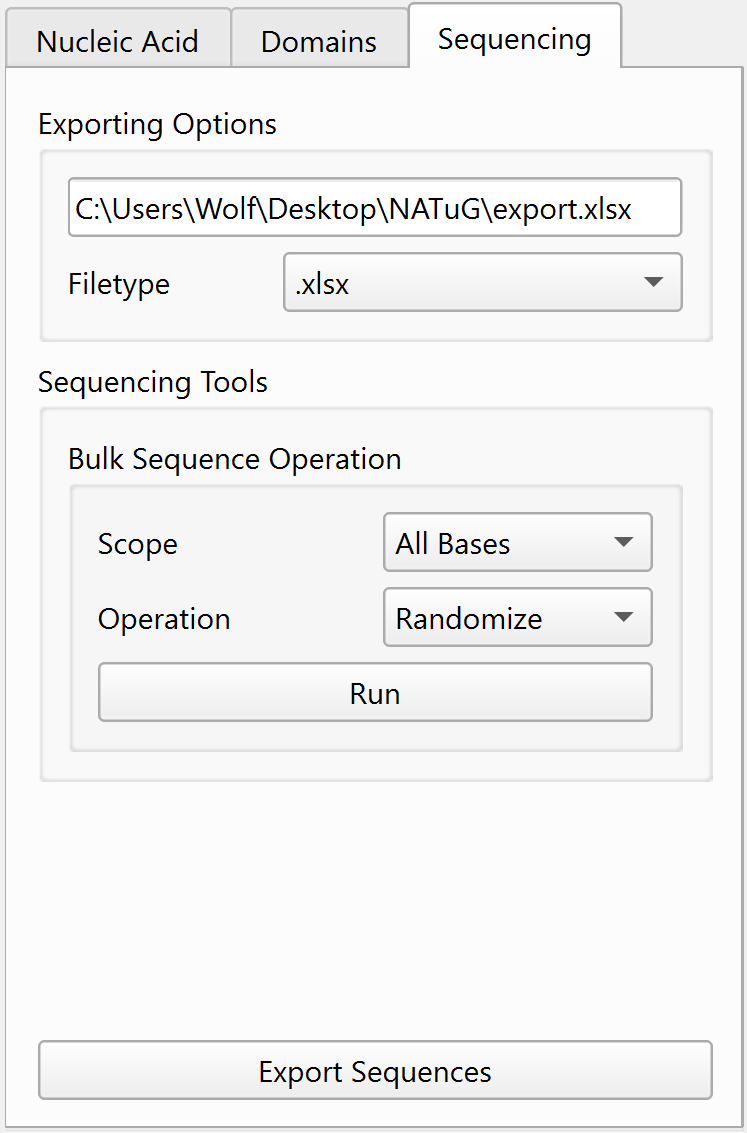
\includegraphics[height=2in]{sequencing-tab.png}
		\label{fig:sequencing-tab}
	\end{figure}
	
	This tab allows for bulk sequence operations, and for exporting sequences to a spreadsheet for synthesis.
	
	\newpage
	
	\subsubsection{Bulk Sequence Operations}
	Bulk sequence operations let you set the sequence of many nucleosides at once. In order to run a bulk sequence operation, select a "Scope," then an "Operation," and then click "Run."
	
	\paragraph{Scopes}
	The scope is which nucleosides the operation should run on.
	
	\begin{itemize}
		\item \textbf{All bases:} All the nucleosides of all the strands.
		\item \textbf{Unset bases:} All the nucleosides of all the strands that do not currently have a base set.
	\end{itemize}

	\paragraph{Operations}
	The operation is what to do to the nucleosides within the scope.
	
	\begin{itemize}
		\item \textbf{Randomize:} Select random bases.
		\item \textbf{Clear:} Unset the bases.
	\end{itemize}
	
	\section{Side View Plot}
	The Side View Plot is the heart of NATuG. It allows you to directly interact with strands that have been created as a result of user inputs set elsewhere. The plot can be broken into a few distinct parts that function together to allow for a high degree of interactivity. 
	
	\begin{figure}[h]
		\centering
		\caption{The Side View Plot \& toolbar}
		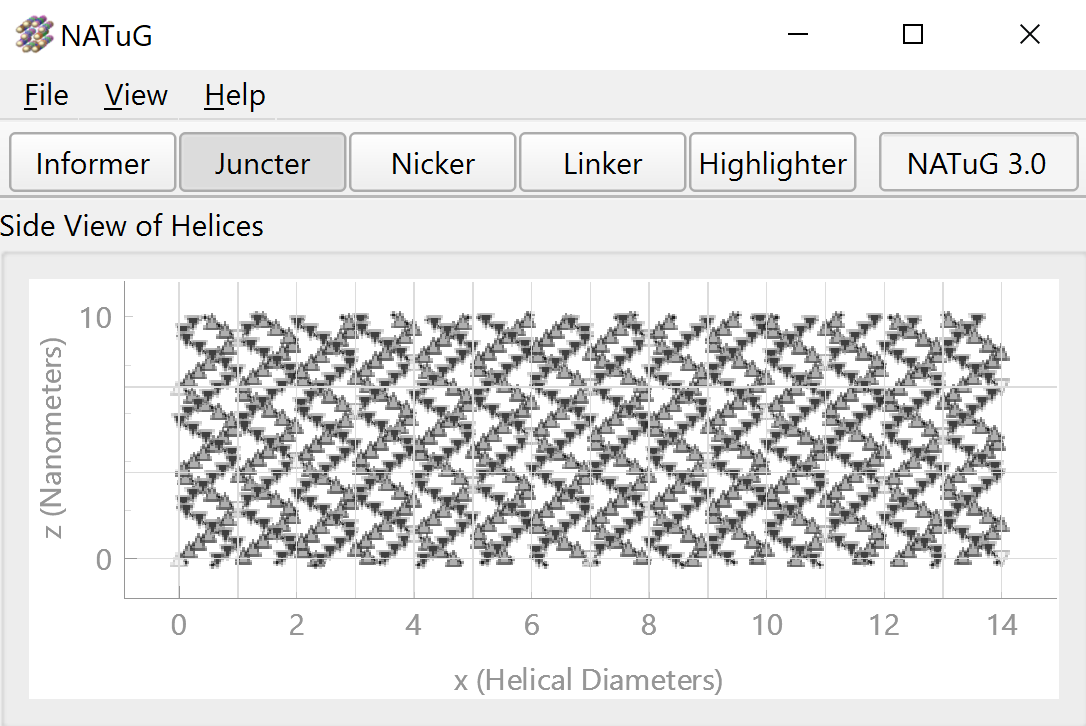
\includegraphics[width=4in]{short-side-view-overview.png}
		\label{fig:short-side-view-overview}
	\end{figure}

	\subsection{Graphics}
	Before diving into how to actually interact with the Side View Plot, it is important to understand what the contents of the plot actually represent. The Side View Plot is not, as its name implies, a direct side view of the double helices. Rather, it is more of an “unrolled” plot, since it is distorted in such a way as to neatly lay out the double helices next to one another.
	
	Importantly, the plot consists of various artifacts, which represent physical nucleosides, or abstract areas between physical nucleosides. Below lies further descriptions of what these artifacts are.
	
	\subsubsection{Points}
	
	\begin{figure}[h]
		\centering
		\caption{Side View Plot Point Graphics}
		\label{fig:side-view-plot-point-graphics}
		
		\begin{subfigure}{.3\linewidth}
			\centering
			
\includegraphics[width=.3in]{up-triangle.png}
			\caption{Triangle Point}
			\label{fig:up-triangle}
		\end{subfigure}%
 		~
		\begin{subfigure}{.3\linewidth}
			\centering
			
\includegraphics[width=.3in]{base-symbol.png}
			\caption{Letter Point}
			\label{fig:base-symbol}
		\end{subfigure}%
		~
		\begin{subfigure}{.3\linewidth}
			\centering
			
\includegraphics[width=.3in]{nondominant-point.png}
			\caption{Circle Point}
			\label{fig:nondominant-point}
		\end{subfigure}
	\end{figure}

	If the Config Panel's (\ref{section:config-panel}) current tab is set to either "Nucleic Acid" or "Domains":
	\begin{itemize}
		\item The triangles represent NEMids. The direction the triangles point (up/down) indicates the direction of the strand. White triangles represent two overlapping NEMids that are clickable, and, when clicked, can form a cross-strand exchange.
		\item The dots represent nucleosides, and cannot be interacted with.
	\end{itemize}

	If the Config Panel's (\ref{section:config-panel}) current tab is set to "Sequencing":
	\begin{itemize}
		\item The triangles represent nucleosides with unset bases. The directions the triangles point (up/down) indicates the direction of the strand.
		\item The letters represent nucleosides that have bases set. The letter indicates what the base of the nucleoside is. 
		\item The dots represent NEMids, and cannot be interacted with.
	\end{itemize}

	\subsubsection{Lines}

	\begin{figure}[h]
		\centering
		\caption{Side View Plot Line Graphics}
		\label{fig:side-view-plot-line-graphics}
		
		\begin{subfigure}{.4\linewidth}
			\centering
			
\includegraphics[width=.3in]{strand-line.png}
			\caption{Strand Line}
			\label{fig:strand-line}
		\end{subfigure}%
		~
		\begin{subfigure}{.3\linewidth}
			\centering
			
\includegraphics[width=.3in]{interdomain-strand-line.png}
			\caption{Interdomain Strand Line}
			\label{fig:interdomain-strand-line}
		\end{subfigure}
	\end{figure}

	The lines connecting dots together are not a literal representation of the location of the phosphate backbone of the DNA, but rather serve as a visual aid to see which strands are which. To this end, by default "interdomain" strands (strands that traverse multiple domains) are automatically styled to be thicker and more colorful to stand out—however, the styles of lines is completely customizable.
	
	Additionally, for interdomain strands, the lines are curved (with \href{https://www.cs.unc.edu/~dm/UNC/COMP258/LECTURES/Chaikins-Algorithm.pdf}{Chaikin's Corner Cutting Algorithm}). This is so that it is clear which strand is which, and because with the thicker lines that interdomain strands posses without corner rounding it becomes unclear at times whether a strand merges with itself. 
	
	\subsection{Interaction}
	NATuG utilizes the pyqtgraph framework for its plots. Below lies a general description of the means of interaction for the plot, but, for a more direct and comprehensive breakdown, visit \href{https://pyqtgraph.readthedocs.io/en/latest/user_guide/mouse_interaction.html}{pyqtgraph’s website} (\href{https://pyqtgraph.readthedocs.io/en/latest/user_guide/mouse_interaction.html}{pyqtgraph.readthedocs.io}).
	
	\subsubsection{Panning}
	To pan from left to right within the side view plot, left click, and then drag your cursor away from the area that you want to pan to. You can think of this as “pulling” the graph towards the cursor. Alternatively, if you have a mouse, you also have the option of clicking the scroll wheel and dragging in the direction that you would like to move the plot in.
	
	\subsubsection{Zooming}
	If you have a mouse:
	\begin{itemize}
		\item To zoom while maintaining the aspect ratio of the plot, use the scroll wheel.
		\item To zoom without regard for the aspect ratio of the plot, right click, and then drag in the direction that you would like to stretch the plot in. The axes will automatically update.
	\end{itemize}
	
	If you have a trackpad:
	\begin{itemize}
		\item To zoom while maintaining the aspect ratio of the plot, pinch inwards to outwards to zoom in, and outwards to inwards to zoom out.
		\item To zoom without regard for the aspect ratio of the plot, pinch and right click simultaneously. 
	\end{itemize}

	\subsubsection{Configuration}
	For additional options for the plot, right click. Upon right clicking, a small dialog showing additional plot options will show up. This allows for more advanced configuration of how the plot appears.
	
	\subsection{Modes}
	The currently chosen mode dictates what left clicks on non-dot points in the Side View Plot does. To change the mode, simply click on the mode that you would like to change to. Only one mode can be chosen at a time, and the currently chosen mode is indicated in a slightly darker gray than the others.
	
	\subsubsection{Informer}
	
	\begin{figure}[h]
		\centering
		\includegraphics[width=3in]{"informer-activated.png"}
		\label{fig:informer-activated}
	\end{figure}

	The "Informer" mode is for obtaining additional information about given points. It provides a dialog that shows various attributes of the point(s) that were clicked on.

	\subsubsection{Juncter}

	\begin{figure}[h]
		\centering
		\includegraphics[width=3in]{"juncter-activated.png"}
		\label{fig:juncter-activated}
	\end{figure}

	The "Juncter" mode allows for the creation of cross-strand exchanges. It lets you click on overlapping NEMids to create junctions.

	\subsubsection{Nicker}

	\begin{figure}[h]
		\centering
		\includegraphics[width=3in]{"nicker-activated.png"}
		\label{fig:nicker-activated}
	\end{figure}

	The "Nicker" mode is how you can create nicks within the strand. Nicks are essentially gaps that split a strand into two different strands.

	\subsubsection{Linker}

	\begin{figure}[h]
		\centering
		\includegraphics[width=3in]{"linker-activated.png"}
		\label{fig:linker-activated}
	\end{figure}

	The "Linker" mode allows you to connect the end of one strand to the beginning of another strand, and vice versa.

	\subsubsection{Highlighter}

	\begin{figure}[h]
		\centering
		\includegraphics[width=3in]{"highlighter-activated.png"}
		\label{fig:highlighter-activated}
	\end{figure}

	The "Highlighter" mode lets you highlight points. It makes them larger and yellow, which can be useful for presentations.
	
	\section{Top View Plot}
	
\end{document}